\documentclass[letter]{article}
\renewcommand{\baselinestretch}{1.25}

\usepackage[margin=1in]{geometry}
\usepackage{physics}
\usepackage{amsmath}
\usepackage{graphicx}
\usepackage{hyperref}


% MATLAB Formating Code
\usepackage[numbered,framed]{matlab-prettifier}
\lstset{style=Matlab-editor,columns=fullflexible}
\renewcommand{\lstlistingname}{Script}
\newcommand{\scriptname}{\lstlistingname}

\allowdisplaybreaks

%opening
\title{MECH 6313 - Homework 1}
\author{Jonas Wagner}
\date{2021, February 1}

\begin{document}

\maketitle


\section{Problem 1}
\textbf{Problem:}
Let
\begin{equation}
	\begin{aligned}
		\dot{x}_1 &= -x_1 + x_2\\
		\dot{x}_2 &= \cfrac{x_1^2}{1 + x_1^2} - 0.5 x_2
	\end{aligned}
\end{equation}

Define an shifted system, linerize that system, and find the center manifold to analyze the stability properties. Then use numerical simulation to plot the phase portrait of the original coordinates and superimpose the shifted center manifold.\\

\textbf{Solution:}
\subsection{Part a}
Let a shifted set of state variables be defined as $\bar{x}_1 = x_1 - 1$ and $\bar{x}_2 = x_2 - 1$. The state variable equation can then be rewritten as
\begin{equation}
	\begin{aligned}
		\dot{\bar{x}}_1 &= -x_1 + x_2\\
		\dot{\bar{x}}_2 &= \cfrac{(\bar{x}_1+1)^2}{(1 + \bar{x}_1^2)^2} - \frac{\bar{x}_2 + 1}{2}
	\end{aligned}
\end{equation}

This system can then be linearized about the origin, resulting in the system matrix
\begin{equation}
	A = \mqty[-1 & 1\\ \frac{1}{2} & -\frac{1}{2}]
\end{equation}
whose eigenvalues are calculated as $\lambda_{1,2} = 0, -\frac{3}{2}$.

A transformation matrix $$T = \mqty[1&-2\\1&1]$$ can then be constructed with the associated eigenvectors to covert into 















\newpage
\section{Problem 2 - S 3.7.3}
\textbf{Problem:}
A simple model of a fishery is given as
\begin{equation}
	\dot{N} = r N (1 - \frac{N}{K}) - H
\end{equation}
where $N$ represents the fish population, $H > 0$ is the number of fish harvested at a constant rate, and both $r$ and $K$ are constants.\\
Redefine the model in terms of $x$, $\tau$, and $h$. Then plot the vector field for various values of $h$. Then identify $h_c$ and classify and discuss the bifurcation.\\

\noindent
\textbf{Solution:}
\subsection{Part a}




Let $x = N / K$, this can then be substituted as
\begin{align}
	\dot{N} = \dv{N}{t} = \dv{x}{t}	
	&= r (K x) \qty(1 - x) - H\\
	\frac{1}{r K} \dv{x}{t}
	&= x \qty(1 - x) - \frac{H}{r K}
	\intertext{Let $h = \frac{H}{r K}$ and $\tau = r K t$,}
	\dv{x}{\tau} &= x (1 - x) - h
\end{align}

\subsection{Part b}

Plotting in matlab


\subsection{Part c}
As is evident by observing the vector fields shown in \ref{fig:pblm1b}, and the bifurcation diagram in \ref{fig:pblm1c}, there exists an $h_c$ where the bifurcation occurs.


\subsection{Part d}
The long time behavior of this model 




\newpage
\section{Problem 3 - S 3.7.4}
\textbf{Problem:}
An improved model of a fishery is given as
\begin{equation}
	\dot{N} = r N (1 - \frac{N}{K}) - H \frac{N}{A + N}
\end{equation}
where $N$ represents the fish population, $H > 0$ is the number of fish harvested at a constant rate, and both $r$, $K$, $A$ are constants.\\
Define the biological interpretation of the parameter $A$. Redefine the model in terms of $x$, $\tau$, and $h$. Find and analyze various fixed points depending on the values of $a$ and $h$. Then analyze the bifurcation that occurs when $h=a$. Then find and classify the other bifurcation that occurs at $h = \frac{1}{4} (a+1)^2$ for $a<a_c$. Finally plot the stability diagram for the system for ($a,h$).\\

\noindent
\textbf{Solution:}
\subsection{Part a}
When a population of fish is being fished, there is a portion of fish that are not possible to catch (such as eggs or fish that are too old).

\subsection{Part b}
Let $x = N / K$, this can then be substituted as
\begin{align}
	\dot{N} = \dv{N}{t} = \dv{x}{t}	
	&= r (K x) \qty(1 - x) - H\frac{K x}{A + K x}\\
	\frac{1}{r K} \dv{x}{t}
	&= x \qty(1 - x) - \frac{H}{r K}\frac{K x}{A + K x}\\
	&= x \qty(1 - x) - \frac{H}{r K}\frac{K x}{K\qty(\frac{A}{K} + x)}\\
	&= x \qty(1 - x) - \frac{H}{r K}\frac{x}{\frac{A}{K} + x}\\
	\intertext{Let $h = \frac{H}{r K}$, $\tau = r K t$, and $a = \frac{A}{K}$}
	\dv{x}{\tau} &= x (1 - x) - h \frac{x}{a + x}
\end{align}

\subsection{Part c}










\newpage
\section{Problem 4 - K 3.8}
\textbf{Problem:}
Let the following system be defined:
\begin{equation}
	\begin{aligned}
		\dot{x}_1 &= -x_1 + \frac{2 x_2}{1 + x_2^2}, \ x_1(0) = a\\
		\dot{x}_2 &= -x_2 + \frac{2 x_1}{1 + x_1^2}, \ x_2(0) = b
	\end{aligned}
\end{equation}
Show that this system has a unique solution for all $t \geq 0$.\\

\noindent
\textbf{Solution:}

The system is known to be continuous on its domain. It is also apparent that both functions are differentiable, which results in a Jacobian of
\begin{equation}
	\mqty[-1		& \cfrac{2}{x_2^2 + 1} - \cfrac{4 x_2^2}{\qty(x_2^2 + 1)^2}\\
		  \cfrac{2}{x_1^2 + 1} - \cfrac{4 x_1^2}{\qty(x_1^2 + 1)^2} & -1]
\end{equation}
which indicates the systems dynamics are both differentiable and differential bounded. This also implies that the system is globbaly Lipshitz continuous, therefore a unique solution exists for $t\geq 0$.

\newpage
\section{Problem 5 - K 3.13}
\textbf{Problem:}
Let the following system be defined:
\begin{equation}
	\begin{aligned}
		\dot{x}_1 &= \tan^{-1}(ax_1) - x_1 x_2\\
		\dot{x}_2 &= b x_1^2 - c x_2
	\end{aligned}
\end{equation}
Derive the sensitivity equations for the parameters vary from their nominal values of $a_0 = 1$, $b_0 = 0$, and $c_0 = 1$. Then simulate the sensitivity equations and the time dependence for the initial conditions of $x_1(0) = 1$ and $x_2(0) = -1$.\\

\noindent
\textbf{Solution:}
\subsection{Part a - Sensitivity Calculation}
Let the following be defined: $$\mu = \mqty[a \\ b \\ c]$$

Let the trajectory $x(\mu, t)$ be defined with regards to parameter changes as:
\begin{equation}
	x(\mu,t) = x(\bar{\mu},t) + \eval{\pdv{x}{\mu}}_{\bar{\mu}} \tilde{\mu}
\end{equation}
where $\tilde{\mu} = \mu - \bar{\mu}$.

It can also be defined by its nonlinear definition as:
\begin{align}
	x(\mu,t) &= x_0 + \int_0^t \dot{x}(x(\mu,\tau), \mu, \tau) \dd{\tau}
	\intertext{The sensativity to the parameters can then be formulated}
	S(t) = \pdv{x}{\mu} &= 0 + \pdv{\mu} \int_0^t f(x(\mu,\tau), \mu, \tau) \dd{\tau}\\
	&=  \int_0^t \pdv{\mu} f(x(\mu,\tau), \mu, \tau) \dd{\tau}\\
	&=  \int_0^t \pdv{f}{x}\pdv{x}{\mu} \pdv{f}{\mu} \dd{\tau}
	\intertext{which can be clculated as jacobians of $f$ resulting in}
	S(t) &=  \int_0^t A(\tau) S(\tau) + B(\tau) \dd{\tau}
\end{align}
where the matrices $A(\tau)$ and $B(\tau)$ are the Jacobians with respect to $x$ and $\mu$ respectively:
\begin{align}
	A(\tau) &= \eval{\pdv{f}{x}}_{\bar{\mu}}  &B(\tau) &= \eval{\pdv{f}{\mu}}_{\bar{\mu}}\nonumber\\
			&= \mqty[-x_2 + \cfrac{x_1}{x_1^2 + 1} 	& - x_1\\
					 0								&1] &
			&= \mqty[\cfrac{x_1}{x_1^2 + 1} & 0 	& 0\\
					 0						& x_1^2 & -x_2]
\end{align}

Finally, the evolution of sensitivity over time can be found using the Leibnitz Formula, resulting in
\begin{equation}
	\dv{s(t)}{t} = A(t) S(t) + B(t)
\end{equation}

\subsection{Part b - Simulation}
The MATLAB code in \appendixname \ref{apx:matlab} simulates and plots the states and sensitivities for each of the parameters. These plots can be seen in \figurename \ref{fig:pblm5}.

\begin{figure}[h]
	\centering
	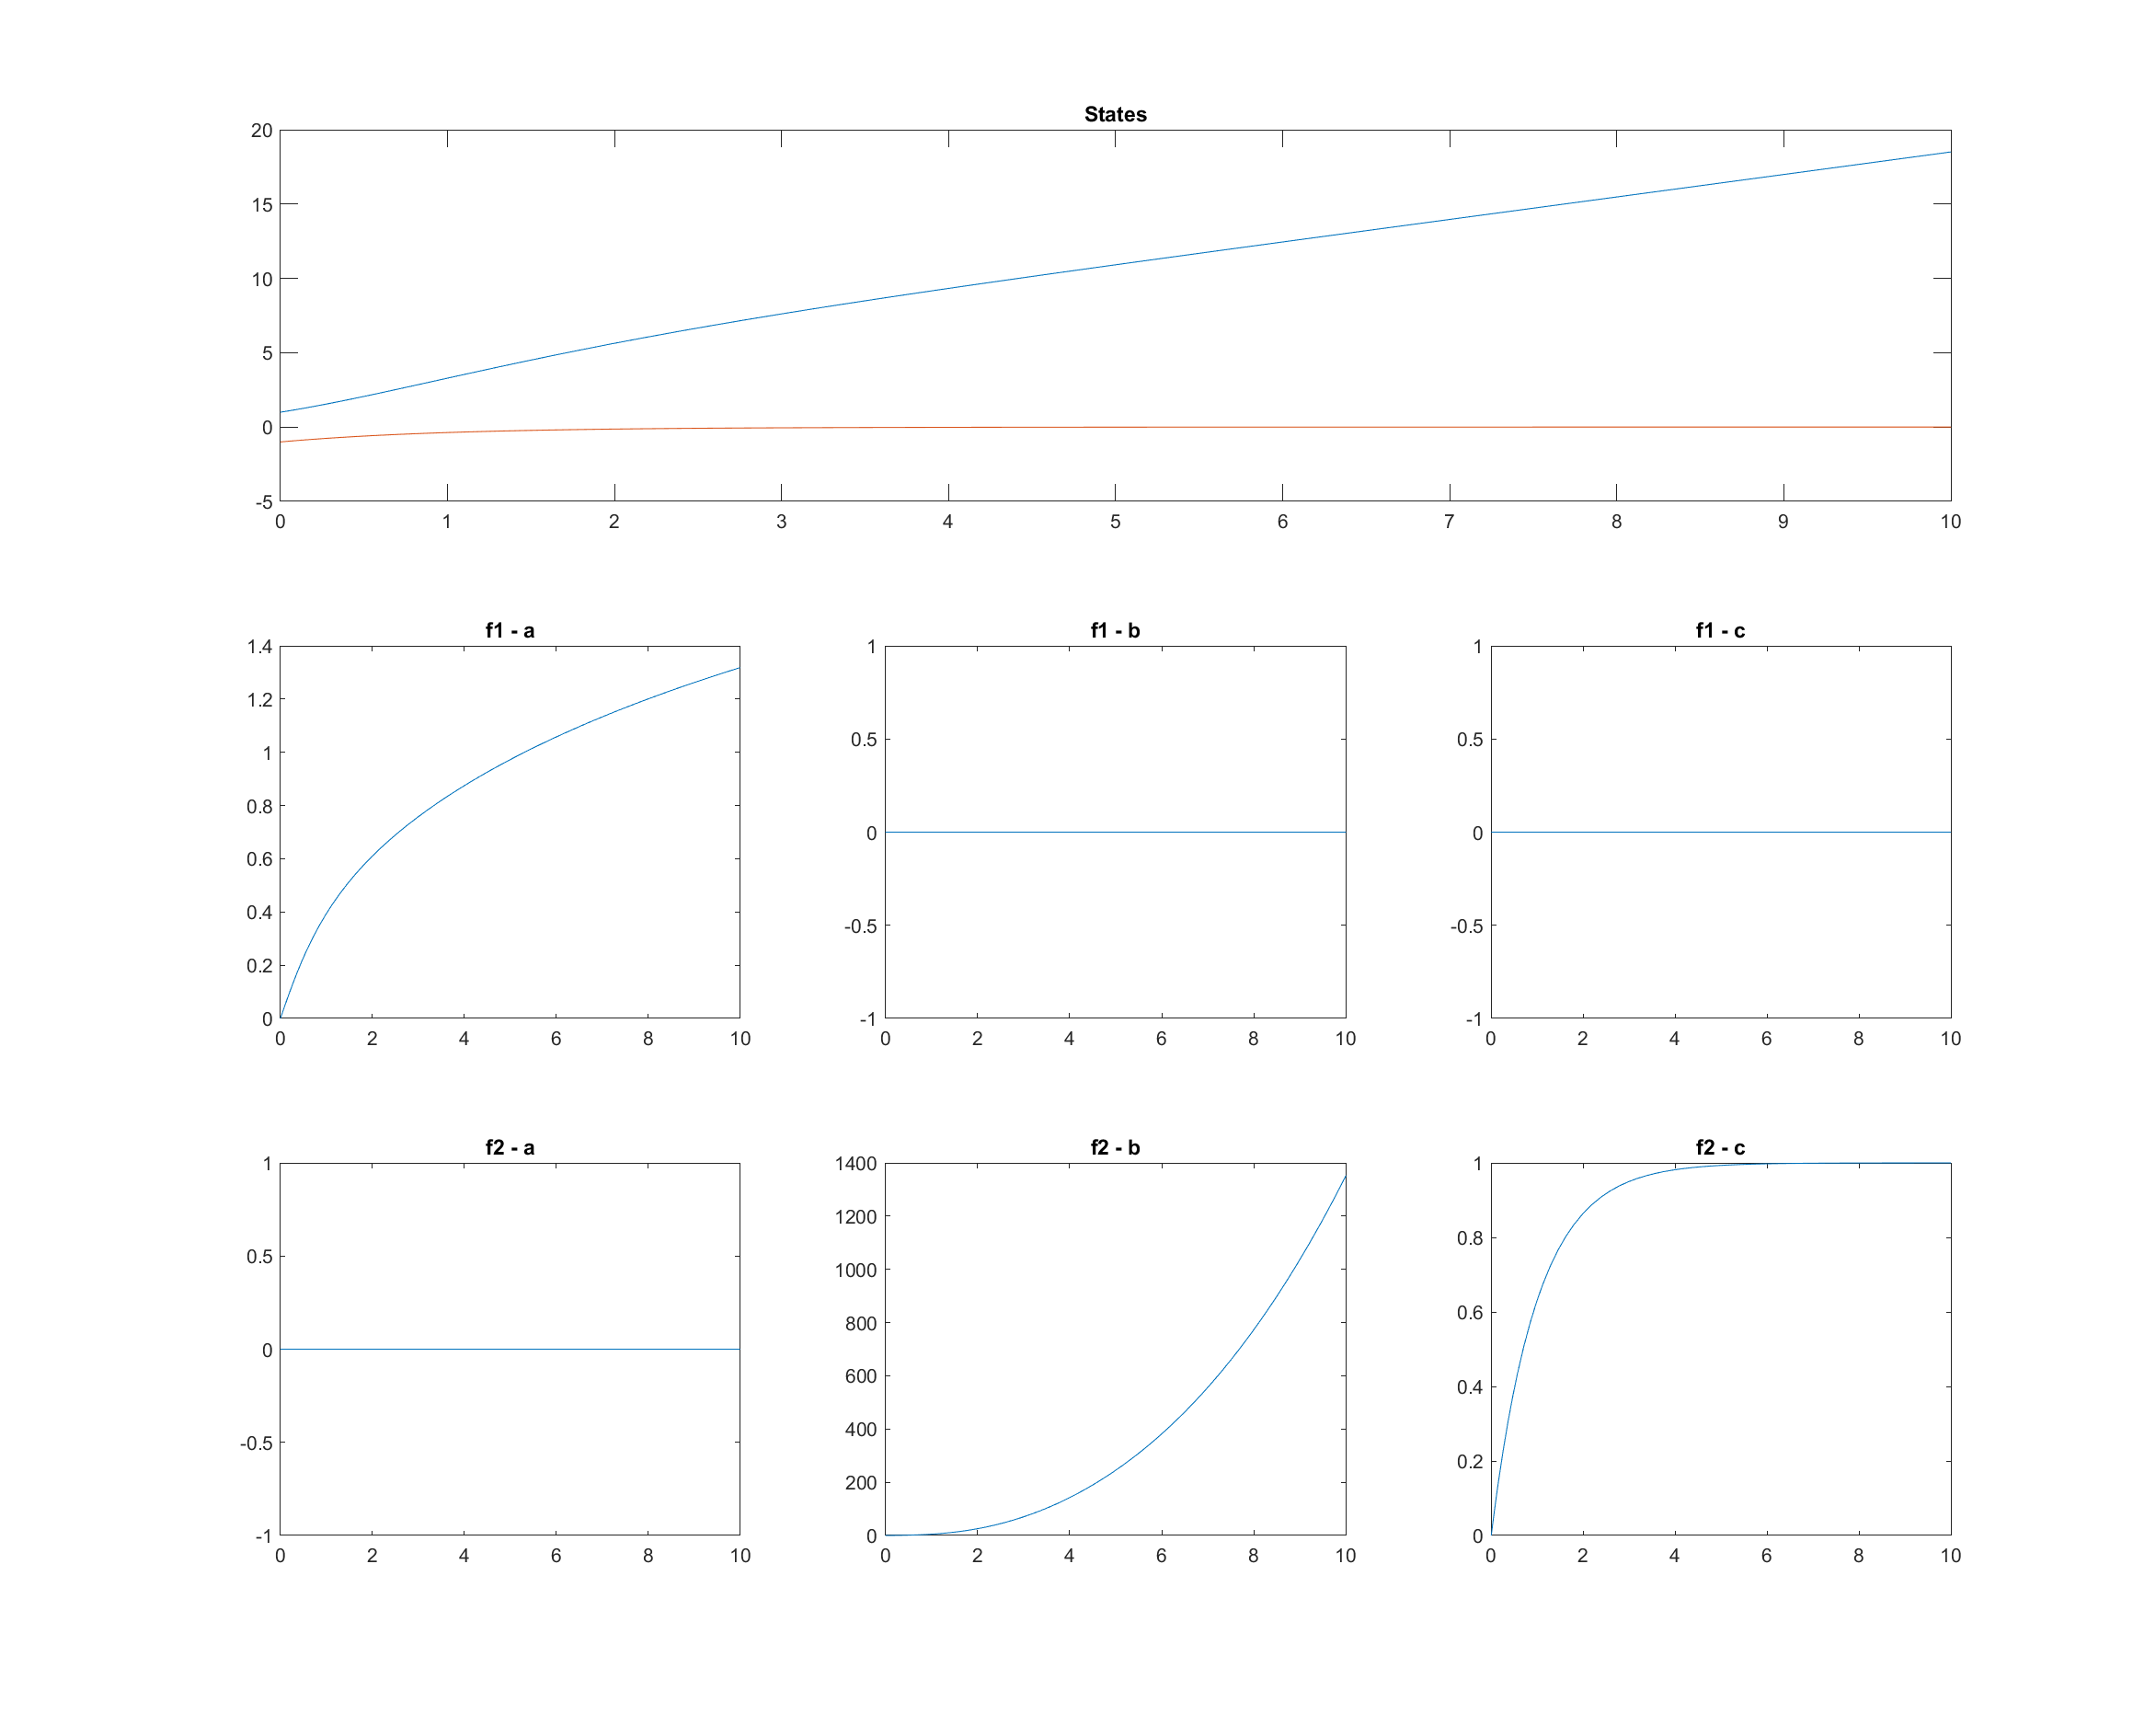
\includegraphics[width=\linewidth]{fig/pblm5}
	\caption{Simulation for Problem 5 with the evolution of sensitivities to parameters.}
	\label{fig:pblm5}
\end{figure}











\newpage
\appendix
\section{MATLAB Code:}\label{apx:matlab}
All code I write in this course can be found on my GitHub repository:\\
\href{https://github.com/jonaswagner2826/MECH6313}{https://github.com/jonaswagner2826/MECH6313}
% MECH6313_HW3
\lstinputlisting[caption={MECH6313\_HW3},label={script:HW1}]{MECH6313_HW3.m}


\end{document}
